\subsection{Kapitel 10}
Die Familie Noahs

\begin{figure}[ht]
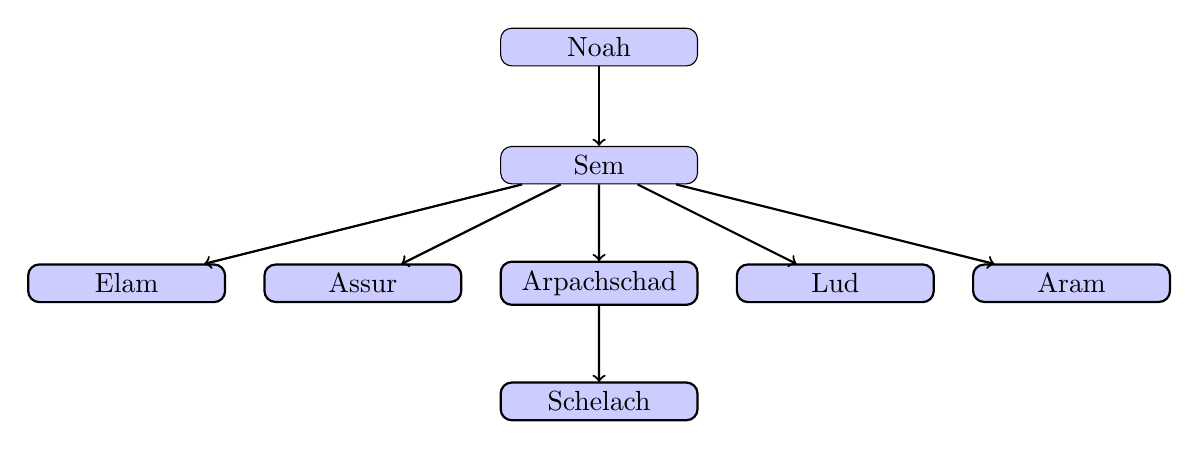
\begin{tikzpicture}
[
    level distance=1.5cm,
    sibling distance=3cm,
    edge from parent/.style={draw,thick, ->},
    every node/.style={draw,rounded corners,fill=blue!20,minimum width=2.5cm,align=center}
  ]

  \node {Noah}
    %child { node {Vater}
      child { node {Sem} 
        child { node {Elam}}
        child { node {Assur}}
        child { node {Arpachschad}
            child { node {Schelach}}
        }
        child { node {Lud}}
        child { node {Aram}}
      }
      %child { node {Ham} }
      %child { node {Jafet} }
    
    %child { node {Onkel} }
    ;
\end{tikzpicture}
\end{figure}